\documentclass[a4paper]{article}
\usepackage[utf8]{inputenc}
\usepackage[spanish, es-tabla, es-noshorthands]{babel}
\usepackage[table,xcdraw]{xcolor}
\usepackage[a4paper, footnotesep = 1cm, width=20cm, top=2.5cm, height=25cm, textwidth=18cm, textheight=25cm]{geometry}
%\geometry{showframe}

\usepackage{tikz}
\usepackage{amsmath}
\usepackage{amsfonts}
\usepackage{amssymb}
\usepackage{float}
\usepackage{graphicx}
\usepackage{caption}
\usepackage{subcaption}
\usepackage{multicol}
\usepackage{multirow}
\setlength{\doublerulesep}{\arrayrulewidth}
\usepackage{booktabs}
\usepackage{mathrsfs,amsmath}
\usepackage{hyperref}
\hypersetup{
    colorlinks=true,
    linkcolor=blue,
    filecolor=magenta,      
    urlcolor=blue,
    citecolor=blue,    
}

\newcommand{\quotes}[1]{``#1''}
\usepackage{array}
\newcolumntype{C}[1]{>{\centering\let\newline\\\arraybackslash\hspace{0pt}}m{#1}}
\usepackage[american]{circuitikz}
\usetikzlibrary{calc}
\usepackage{fancyhdr}
\usepackage{units} 

\graphicspath{./Imagenes}

\pagestyle{fancy}
\fancyhf{}
\lhead{22.05 ASSD}
\rhead{Mechoulam, Lambertucci, Rodriguez, Londero}
\rfoot{Página \thepage}

\begin{document}

\subsection{Introducción modelo Karplus-Strong}
En esta sección se analizará el método de síntesis basado en el modelado físico, propuesto por Karplus-Strong.
\subsection{Karplus-Strong básico}
El modelo básico de Karplus-Strong consiste filtrar una forma de onda a travez de una linea de retardo, gracias a esto se logra simular el sonido de una cuerda de guitarra.
\begin{figure}[H]
	\centering
	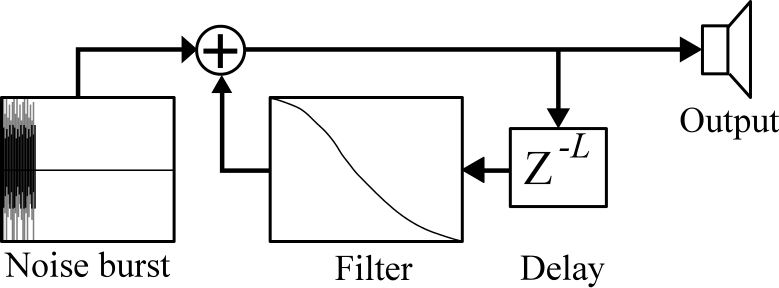
\includegraphics[width=0.8\textwidth]{ImagenesEjercicio4/ksinit.PNG}
\caption{Modelo clásico Karplus-Strong.}
	\label{fig:kscl}
\end{figure}
\subsubsection{Análisis teórico}
Este algoritmo se puede describir por su diagrama en bloques como se ve  a continuación.
\begin{figure}[H]
	\centering
	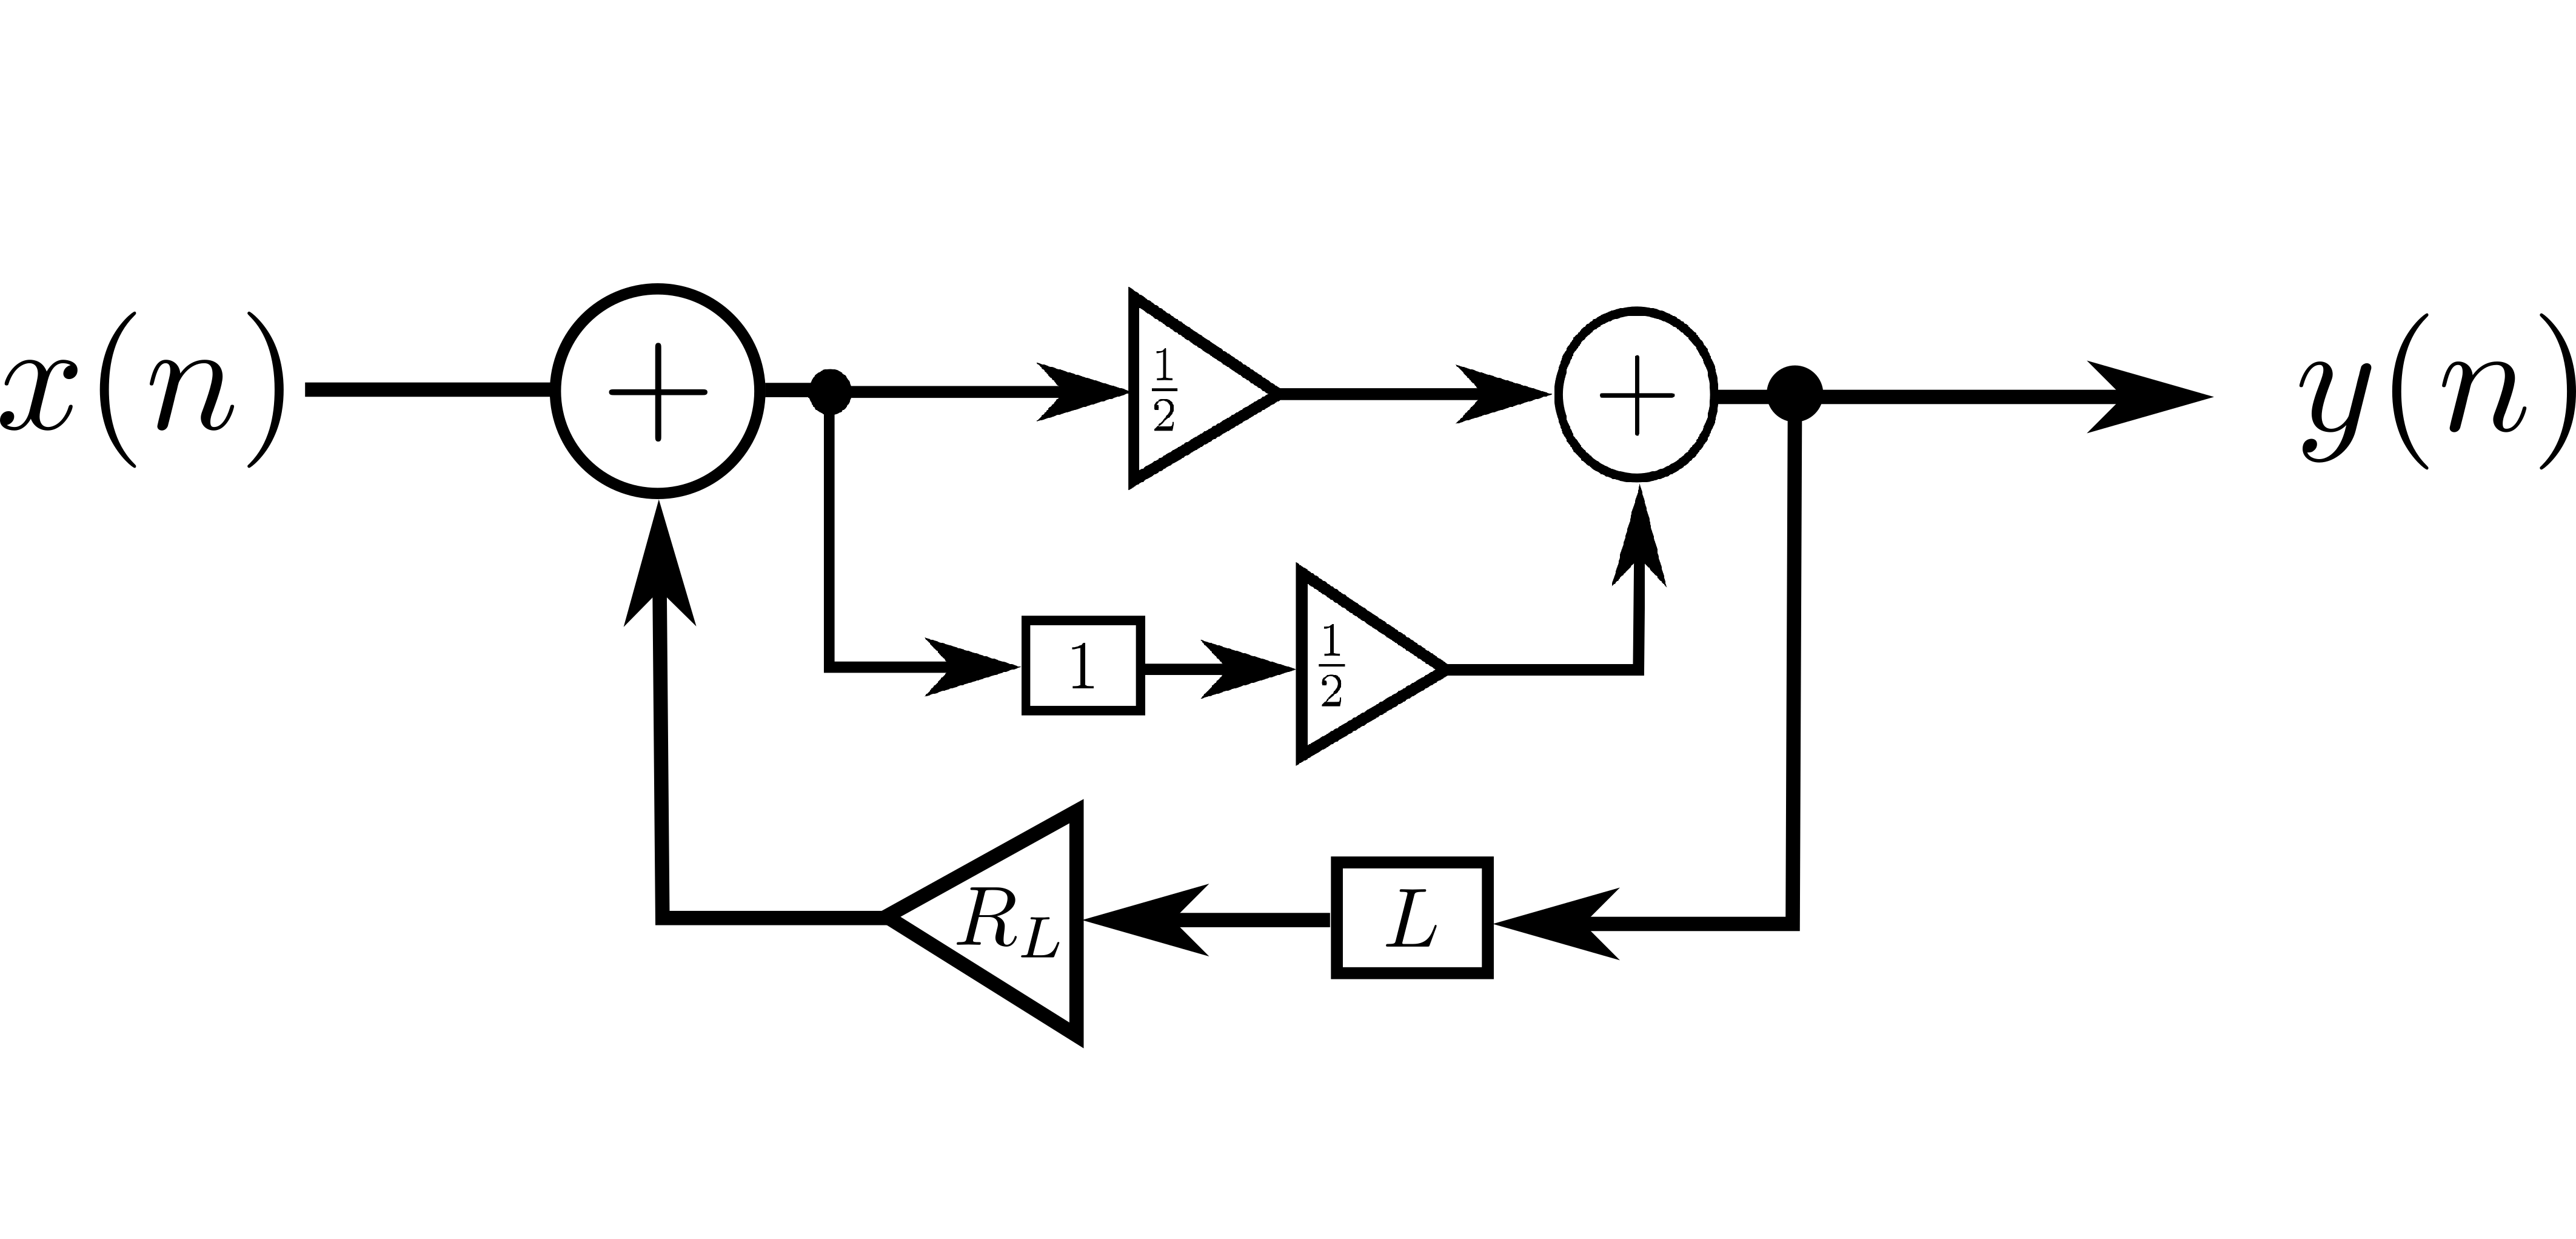
\includegraphics[width=0.8\textwidth]{ImagenesEjercicio4/ksclasic.PNG}
\caption{Algoritmo Karplus-Strong.}
	\label{fig:ksclasico}
\end{figure}
De este diagrama en bloques se puede obtener la ecuación en diferencias:
\begin{align}
y(n) = \frac{1}{2}\cdot x(n) +\frac{1}{2}\cdot x(n-1) + \frac{1}{2}\cdot R_L \cdot y(n-L) + \frac{1}{2}\cdot R_L \cdot y(n-L-1) 
\label{eq:eqdif}
\end{align}
A partir de esta expresión se puede calcular su transformada Z y despejar para la transferencia:
\begin{align}
H(z) = \frac{\frac{1}{2} \cdot z^{L+1} +\frac{1}{2} \cdot z^{L} }{z^{L+1} - \frac{R_L}{2} \cdot z - \frac{R_L}{2}}
\label{eq:hzks}
\end{align}  
Vale la pena mencionar que de la ecuación (\ref{eq:eqdif}) es una ecuación en diferencias que cuenta como condiciones iniciales la wavetable suministrada por el ruido.
\subsubsection{Análisis singularidades}
Se observa que la expresión (\ref{eq:hzks}) cuenta con L+1 polos y L+1 ceros (de los cuales L de esos ceros se encuentran en el origen). A continuación se muestra un diagrama de polos y ceros del sistema:
\begin{figure}[H]
	\centering
	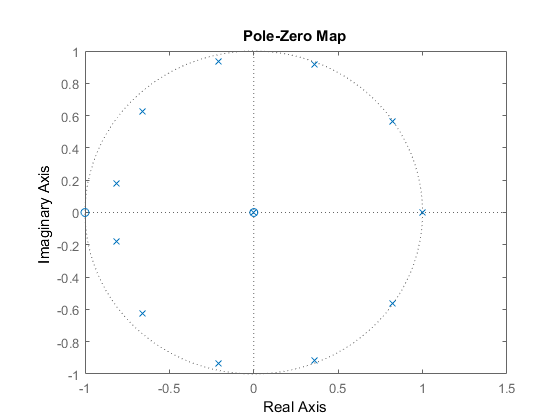
\includegraphics[width=0.8\textwidth]{ImagenesEjercicio4/pzks.PNG}
\caption{Diagrama de polos y ceros.}
	\label{fig:zpdig}
\end{figure}
Adicionalmente se graficó el diagrama de bode del sistema.
\begin{figure}[H]
	\centering
	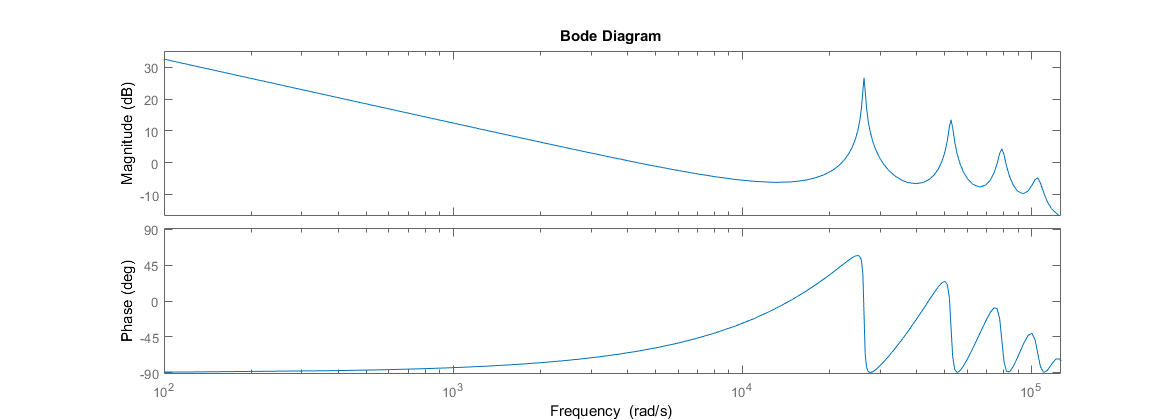
\includegraphics[width=\textwidth]{ImagenesEjercicio4/bodeks.PNG}
\caption{Diagrama de Bode.}

	\label{fig:bode}
\end{figure}
Considerando que los parámetros eran: $f_s = 44.1kHz$, $L=10$ y $R_L=1$
\subsubsection{Sintonización de frecuencia}
En cuanto a la elección de una frecuencia de oscilación se puede observar en los úlitmos gráficos que existe un valor de frecuencia, la cual tiene mayor probabilidad de cumplir el criterio de Barkhausen, la cual corresponde a $f_r = \frac{f_s}{L+0.5}$, esto se debe a que el sistema es la superposición de una linea de retraso  L y otra sistema de retraso L+1, la señal al recorrer el lazo lo hace cada $\frac{L+L+1}{2}$ cambiando esto por frecuencia se obtiene:
\begin{align}
f_r=\frac{f_s}{L+0.5}
\label{eq:fr}
\end{align}
\subsubsection{Tipos de ruido}
Se propuso excitar el sistema con distintos tipos de ruido de entrada, siendo estos:
\begin{itemize}
\item Ruido Gaussiano
\item Ruido Uniforme
\item Ruido Binario
\end{itemize}
Primero se aplico ruido gaussiano de longitud L=50, y se obtuvo la siguiente salida:
\begin{figure}[H]
	\centering
	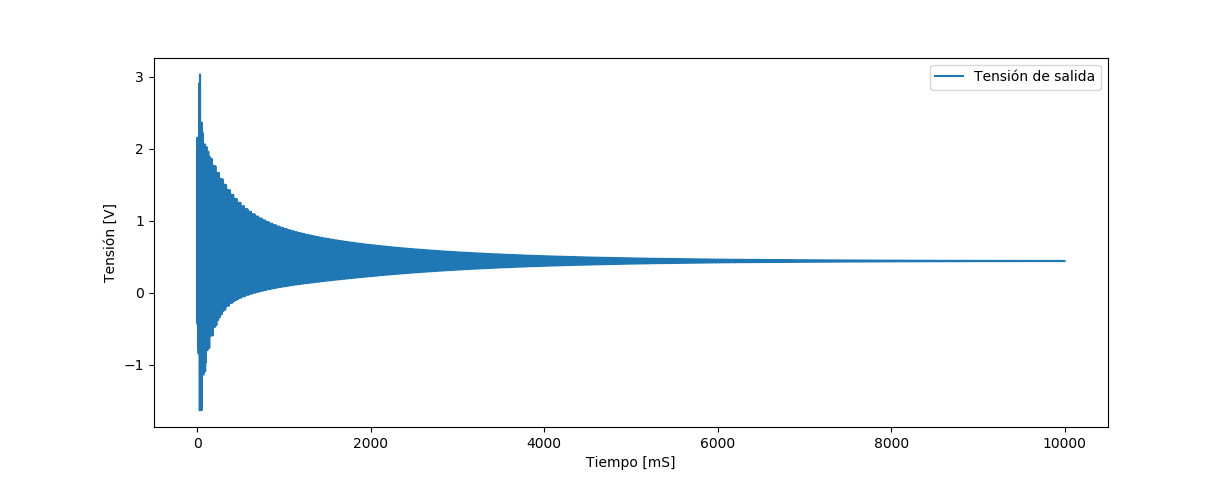
\includegraphics[width=\textwidth]{ImagenesEjercicio4/gaussianResponse.PNG}
\caption{Respuesta a ruido gaussiano, L=50.}
	\label{fig:gaussiano}
\end{figure}
Se puede apreciar que la respuesta al ruido gausiano, parece tener cierta simetría respecto al eje.
Algo notable es mencionar como el sistema se estabiliza para un valor levemente superior a 0. 
adicionalmente se realizó un detalle en la foto:
\begin{figure}[H]
	\centering
	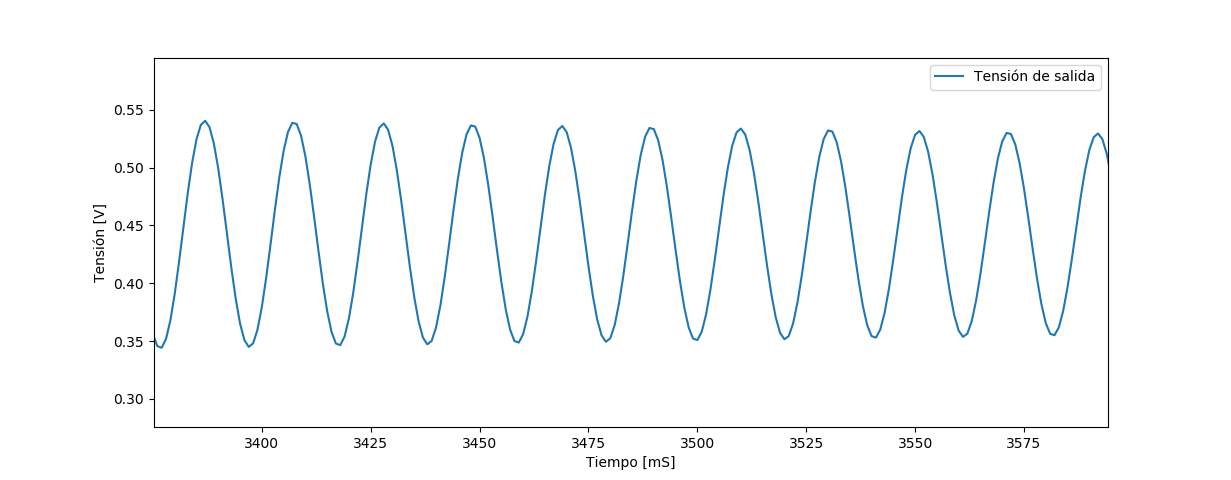
\includegraphics[width=\textwidth]{ImagenesEjercicio4/gaussianResponseDETAIL.PNG}
\caption{Respuesta a ruido gaussiano detalle, L=50.}
	\label{fig:gaussianod}
\end{figure}
Aquí se puede apreciar que el sistema efectivamente se encuentra oscilando , mientras siendo atenuado por una envolvente.\\
Luego se excitó el sistema con ruido uniforme, obteniendo la siguiente respuesta:
\begin{figure}[H]
	\centering
	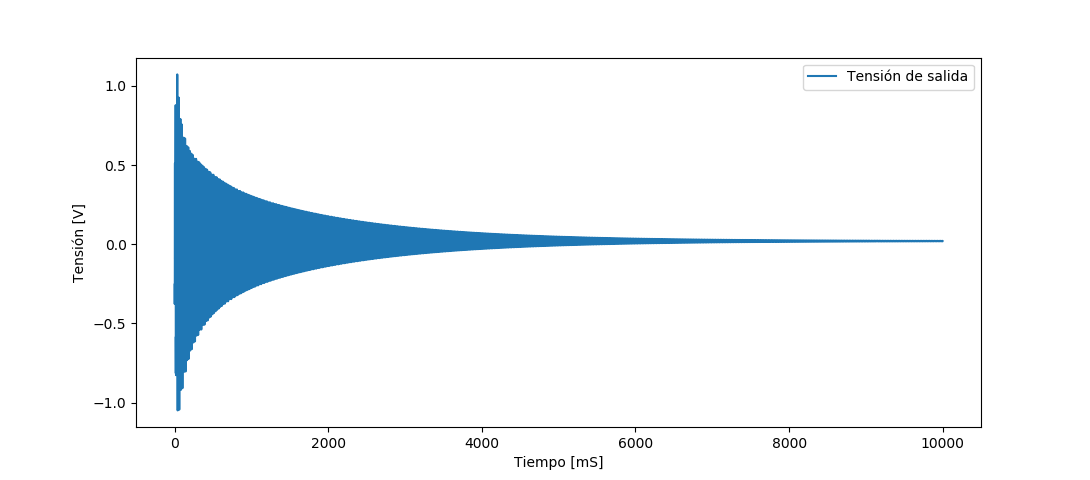
\includegraphics[width=\textwidth]{ImagenesEjercicio4/uniformResponse.PNG}
\caption{Respuesta a ruido uniforme, L=50.}
	\label{fig:uniforme}
\end{figure}
Se puede apreciar que la respuesta al ruido uniforme, cuenta con una simetría respecto al eje mas notable que el gausiano, y un tiempo de decay mas lento, adicionalmente el valor al que tiende es mucho mas cercano a cero.

adicionalmente se realizó un detalle en la foto:
\begin{figure}[H]
	\centering
	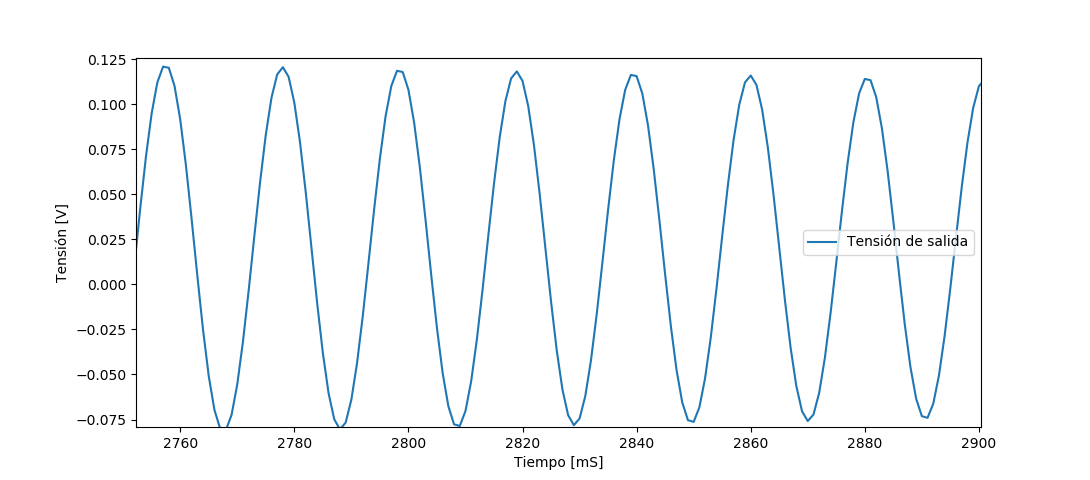
\includegraphics[width=\textwidth]{ImagenesEjercicio4/uniformResponseDETAIL.PNG}
\caption{Respuesta a ruido uniforme detalle, L=50.}
	\label{fig:uniformed}
\end{figure}
Finalmente se ingresó al sistema con ruido Binario aleatorio.
\begin{figure}[H]
	\centering
	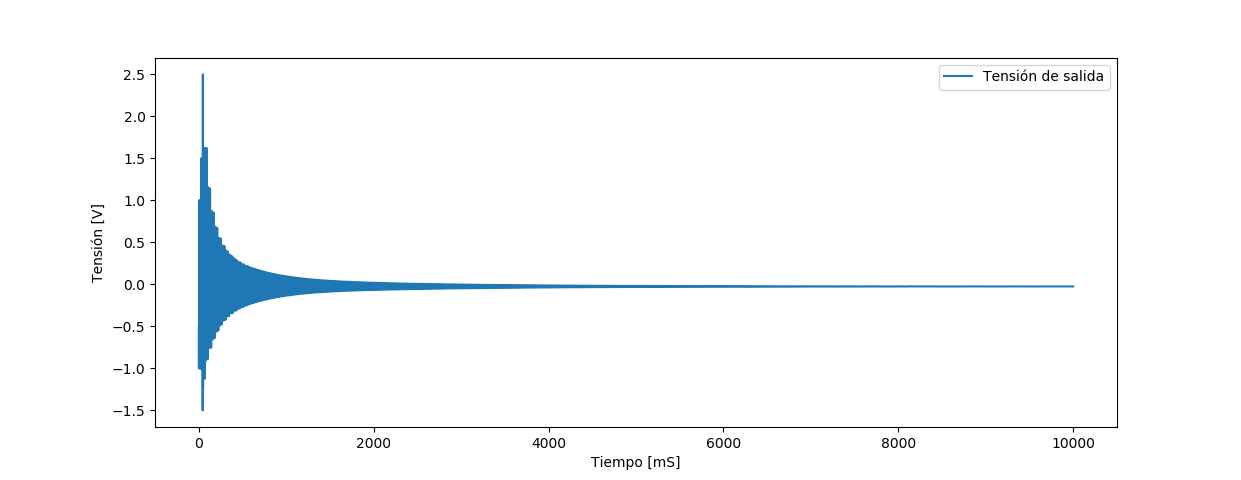
\includegraphics[width=\textwidth]{ImagenesEjercicio4/binaryResponse.PNG}
\caption{Respuesta a ruido Binario, L=50.}
	\label{fig:binary}
\end{figure}
Se puede observar en la figura que tiene una envolvente mucho mas severa que las anteriores, y que cuando el tiempo aumenta tiende cercano a cero el valor de tensión lo cual es deseado.
\begin{figure}[H]
	\centering
	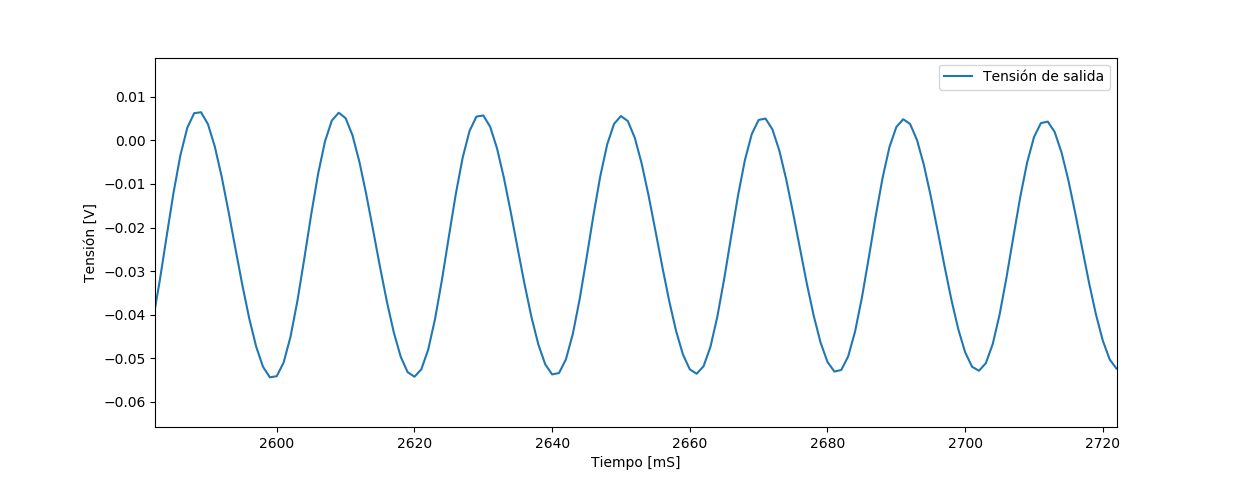
\includegraphics[width=\textwidth]{ImagenesEjercicio4/binaryResponseDETAIL.PNG}
\caption{Respuesta a ruido Binario en detalle , L=50.}
	\label{fig:binaryD}
\end{figure}
Adicionalmente se computó la respuesta impulsiva del sistema, siendo esta:
\begin{figure}[H]
	\centering
	\includegraphics[width=\textwidth]{ImagenesEjercicio4/impulseResponse.PNG}
\caption{Respuesta al Impulso, L=50.}
	\label{fig:impulse}
\end{figure}
Vale la pena mencionar que la salida nunca es negativa, esto se debe a que cuando la excitación es únicamente positiva, dado que la realimentación es positiva, y no existe ninguna inversión de fase, la salida siempre será positiva.
Asi también se muestra un detalle de la respuesta.
\begin{figure}[H]
	\centering
	\includegraphics[width=\textwidth]{ImagenesEjercicio4/impulseResponseDETAIL.PNG}
\caption{Respuesta al Impulso detalle, L=50.}
	\label{fig:impulsed}
\end{figure}
\subsubsection{Estabilidad}
La estabilidad del sistema será determinada por la ecuación (\ref{eq:hzks}) se puede observar que si RL es mayor o igual a uno el sistema será inestable, si bien teóricamente esto es cierto, en la realidad se encuentra que si RL = 1 no solo no provocará inestabilidad, sino que es recomendable este valor dado que logrará extender las oscilaciones  un mayor tiempo.
\subsection{Mejora propuesta}
El sistema anterior contaba con algunas limitaciones, un claro ejemplo de esto es la frecuencia,
que para valores pequeños de L la diferencia entre $f_r(L)$ y $f_r(L+1)$ resulta grande, dejando una banda de frecuencias sin poder ser sintonizadas, como ejemplifica la siguiente imagen.
\begin{figure}[H]
	\centering
	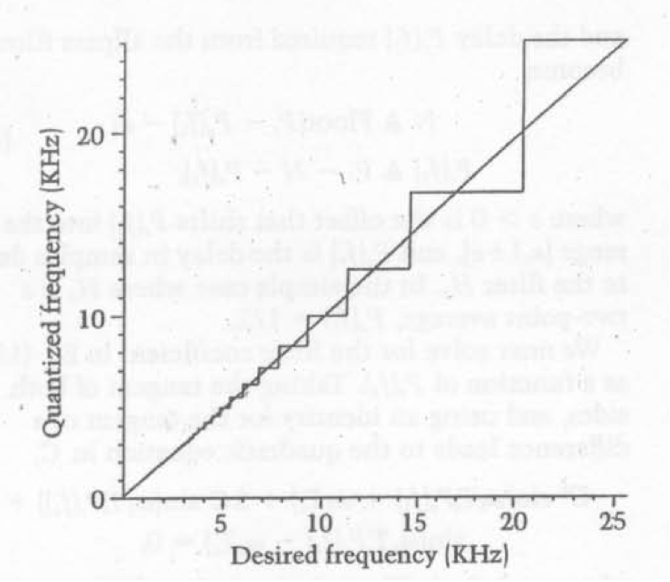
\includegraphics[width=0.6\textwidth]{ImagenesEjercicio4/sintfreq.PNG}
\caption{Dificultad en sintonización de frecuencia.}
	\label{fig:sintfreq}
\end{figure}
Otro defecto, es el final abrupto con el que cuentan algunas notas, si se pide una duración reducida, ya que las discontinuidades en el sonido provocan un efecto indeseado.
\subsubsection{Sintonización de frecuencia}
Para definir la frecuencia  de resonancia del sistema, dado que la ecuación (\ref{eq:fr}) no deja grados de libertad, ya que la frecuencia de muestreo es fija, lo único que se puede hacer es realizar una modificación al circuito. El nuevo modelo propuesto es el siguiente:
\begin{figure}[H]
	\centering
	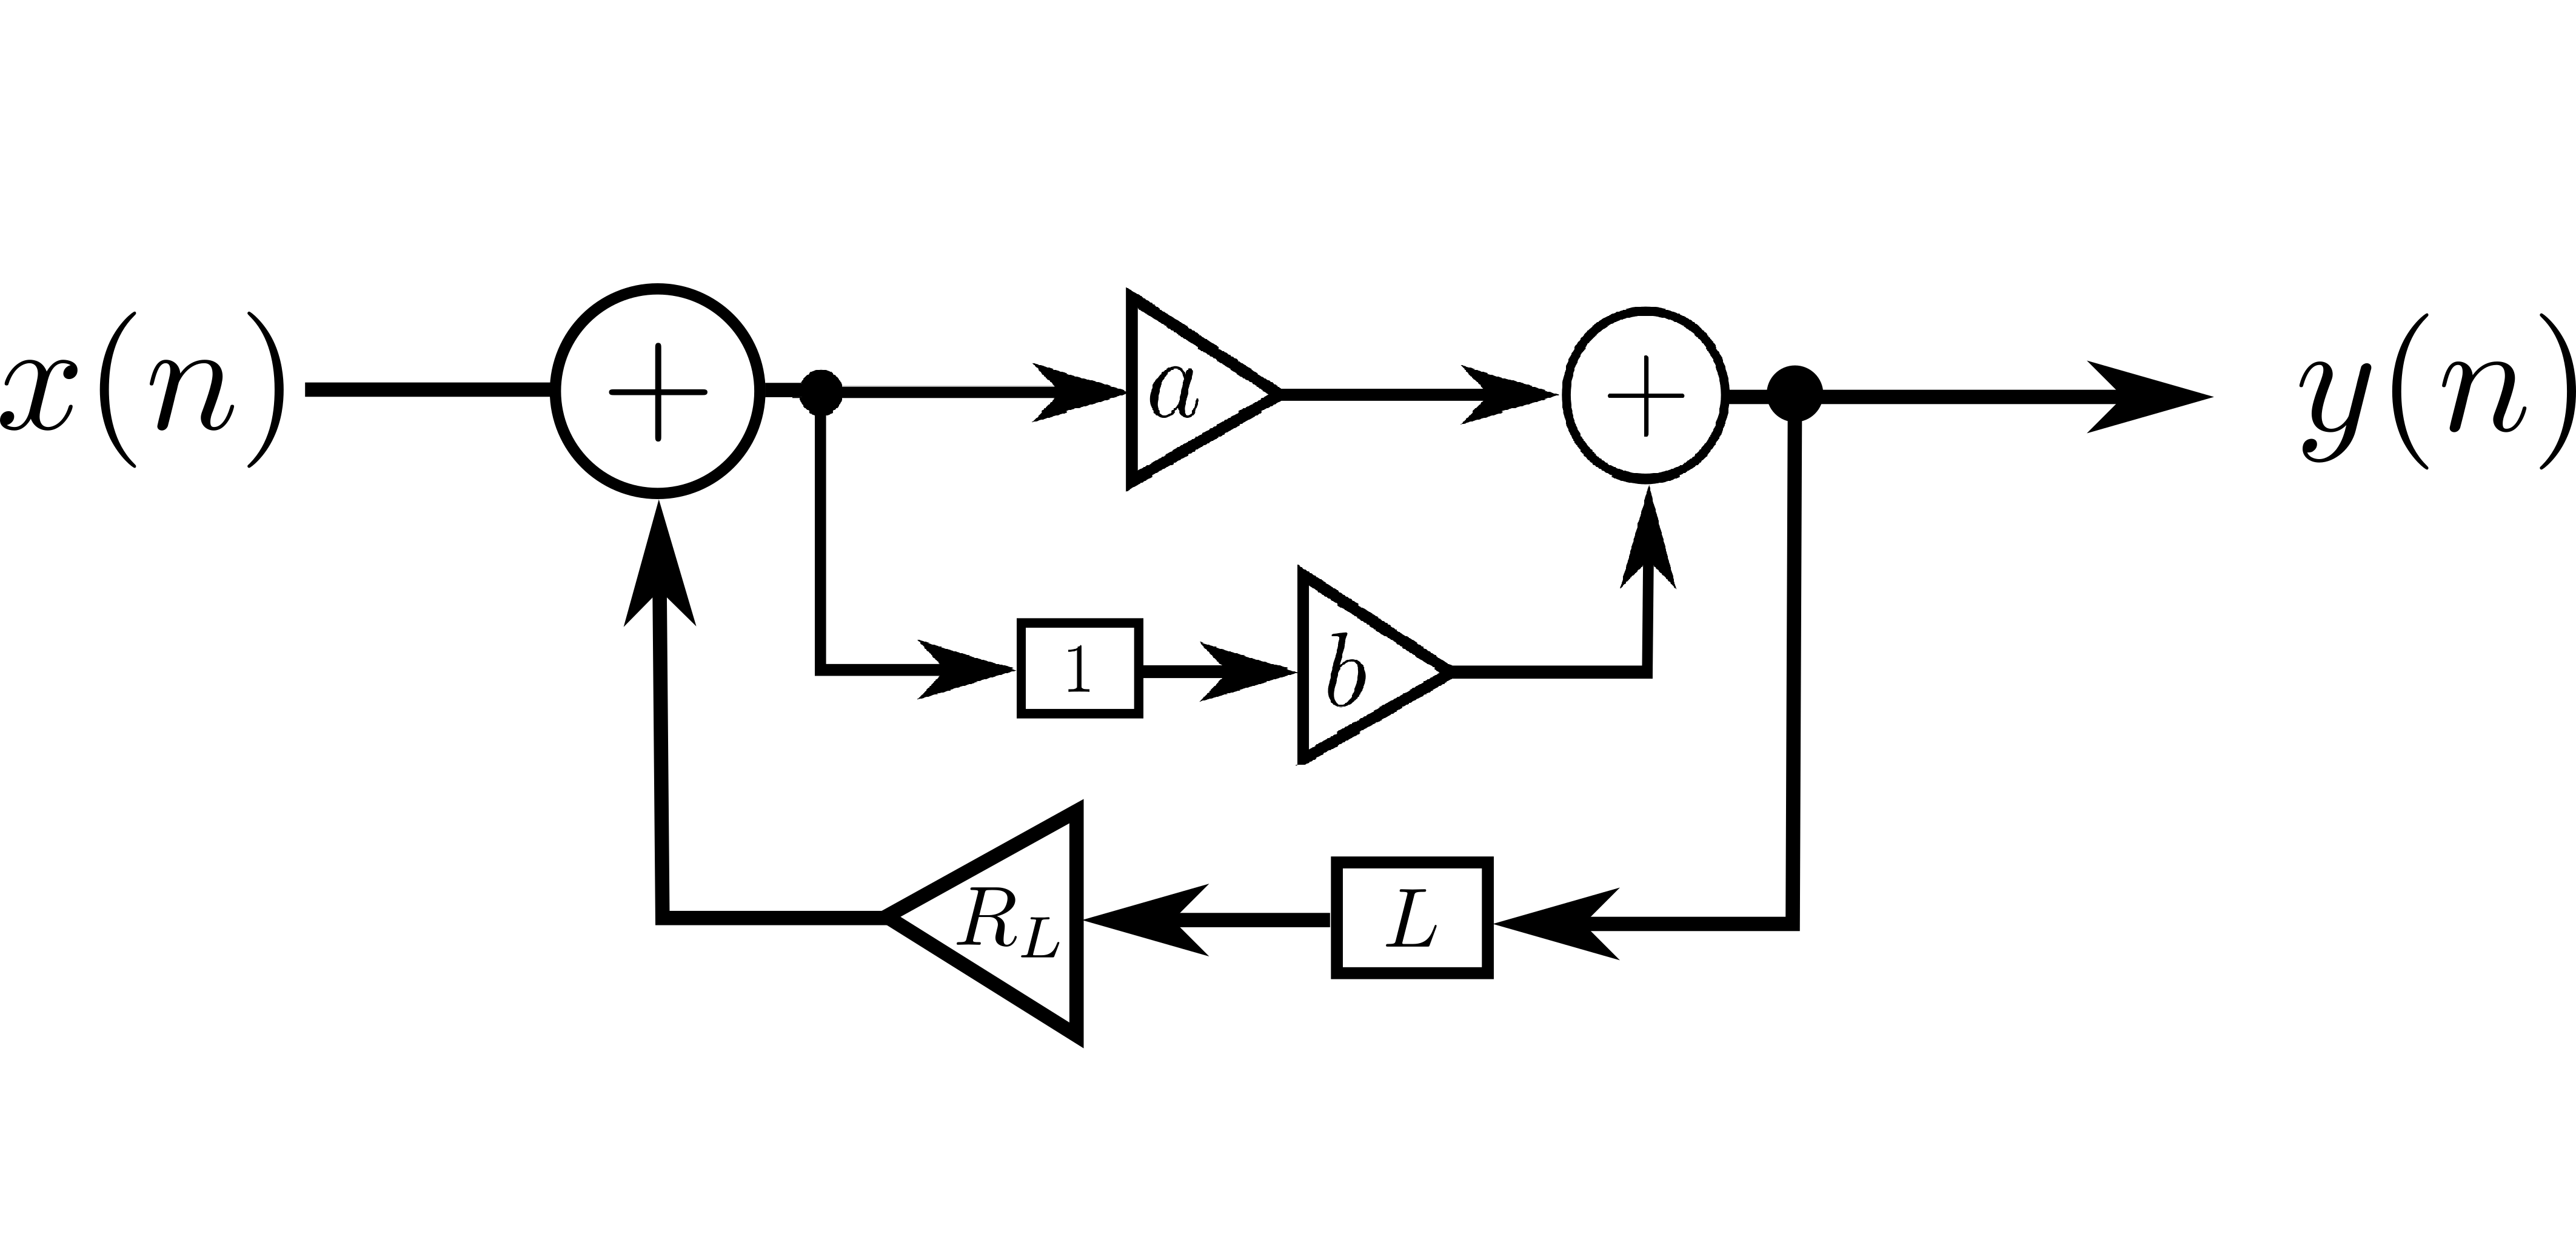
\includegraphics[width=0.8\textwidth]{ImagenesEjercicio4/mejoraks.PNG}
\caption{Algoritmo Karplus-Strong mejora propuesta.}
	\label{fig:ksmejora}
\end{figure}
Utilizando esta propuesta se puede obtener la ecuación en diferencias del sistema, siendo esta:
\begin{align}
y(n) = a\cdot x(n) +b\cdot x(n-1) + a\cdot R_L \cdot y(n-L)+b\cdot R_L \cdot y(n-L-1) 
\end{align}
Notese, que si $a=b=$ $\frac{1}{2}$ el sistema coincide con el original.
Utilizando el mismo razonamiento que fue utilizado anteriormente, se llega a que la nueva frecuencia de resonancia será:
\begin{align}
f_r=\frac{f_s}{L\cdot (a+b)+b}
\end{align}
eligiendo apropiadamente a y b, y teniendo en cuenta que su suma debe de dar 1 para que el sistema sea el promedio ponderado realizado por estos sea realmente un promedio.\\
Un punto en contra de esta solución es que dependiendo de los valores de a y b se toma mas en consideración una u otra linea del promedio.
\subsubsection{Continuidad del sonido}
Se tuvo en cuenta que el sonido sea una función suave, dado que cambios bruscos en el sonido no son placenteros ni esperados en la sintetización que deseamos implementar, para lidiar con este problema lo que se realizo fue definir un factor de ventana, a partir de la cual una ventana atenuaría gradualmente el sonido hasta que sea nulo, para esto se definió una ventana, que tendrá valor unitario para valores de tiempo menores al factor de ventana especificado, y para valores superiores, decaerá gradualmente con una función cosenoidal, barriendo desde 0 a $\frac{\pi}{2}$ como se ilustra a continuación.
\begin{figure}[H]
	\centering
	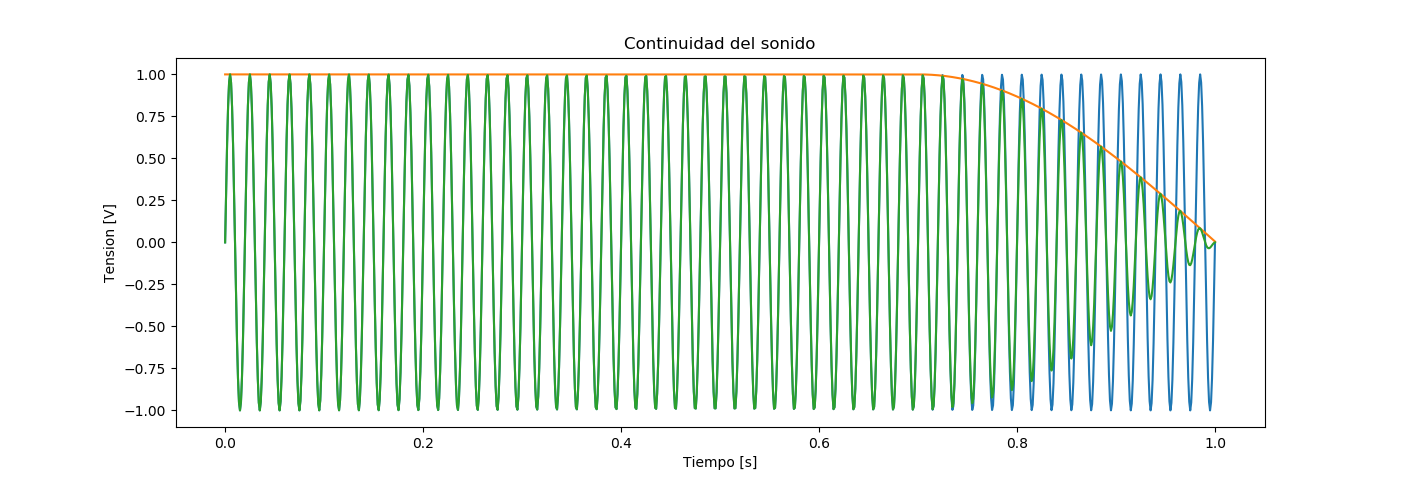
\includegraphics[width=1\textwidth]{ImagenesEjercicio4/continuidad.PNG}
\caption{Muestra del factor de ventana.}
	\label{fig:windowfactor}
\end{figure}
Esto aumenta la calidad de la síntesis en gran medida si se combina con la idea de que la duración de la nota y la del sonido son cosas distintas.
\subsubsection{Caja de resonancia}
La caja de resonancia es una parte primordial de la gran mayoría de instrumentos acústicos, principalmente de cuerda y percusión, que tiene la finalidad de amplificar o modular un sonido (en los instrumentos de cuerda generalmente a través de un puente). 
Los instrumentos que cubren rangos de sonidos más graves, como el contrabajo, el violonchelo o el bombo, necesitan una caja de resonancia bastante mayor que el resto.
La necesidad de utilizar una caja de resonancia en una guitarra se debe justamente a que la vibración de las cuerdas, que generan los frente de onda esféricos propios del sonido, tienen una gran dificutad para propagarse por el medio (el aire) debido a su reducida amplitud. La manera elegida de sopesar este problema suele ser la utilización de una caja de resonancia, esta cumple la función de capturar parte del frente de onda en su cavidad, allí las frecuencias producidas por las cuerdas son amplificadas en igual magnitud y luego liberadas al medio, ahora con la intesidad suficienste para que pueda propagarse y que sea apreciable el sonido.\\
Finalmente cabe destacar que en el ámbito de señales realmente no es necesario dicha caja, al igual que tampoco un filtro que la emule, debido a que su función es amplificar, y eso se puede hacer digitalmente sin ningún problema. 


\subsection{Karplus-Strong percusión}
Se puede realizar una modificación al modelo inicial agregando un factor aleatorio como se observa a continuación:
\begin{figure}[H]
	\centering
	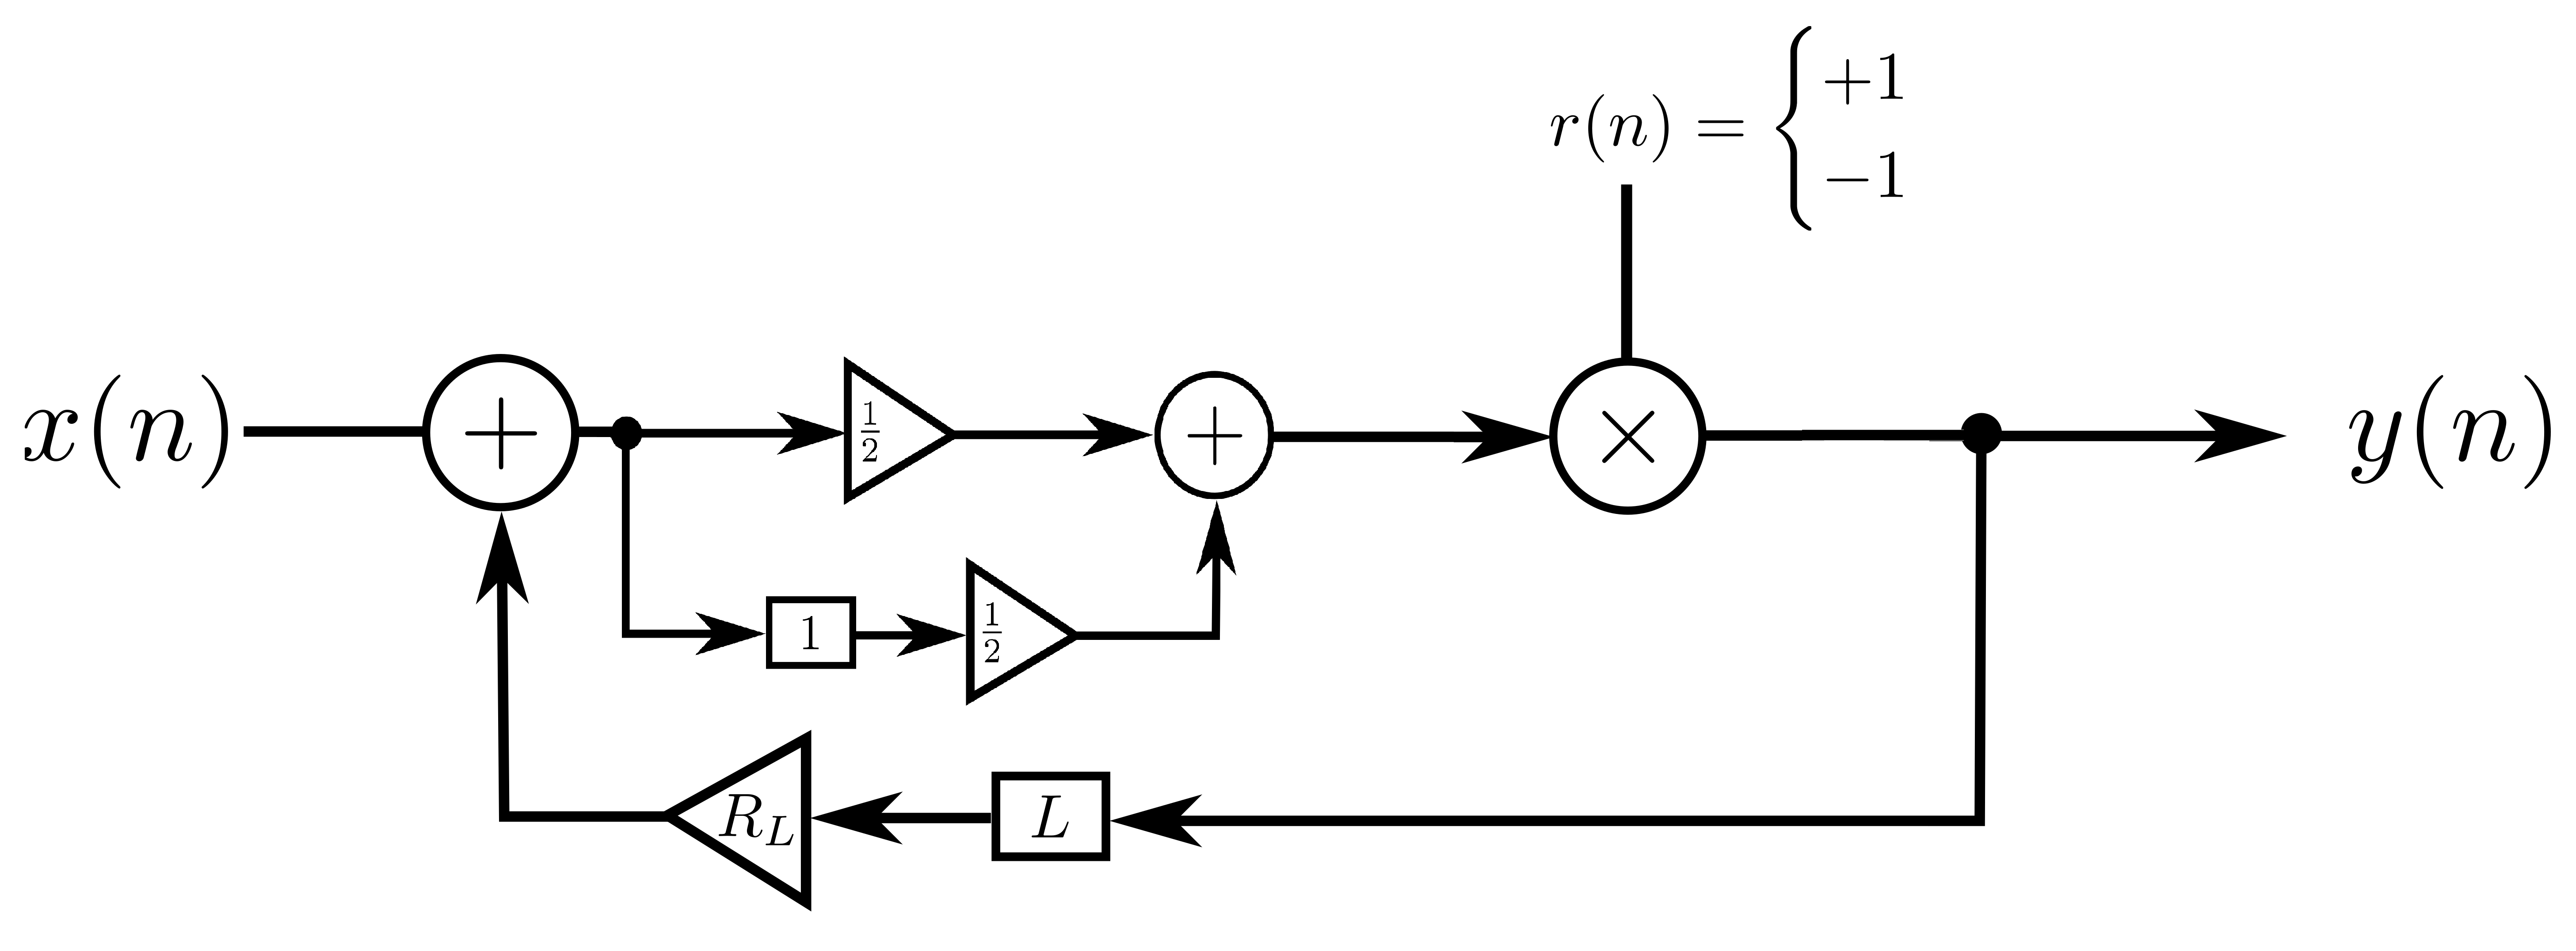
\includegraphics[width=1\textwidth]{ImagenesEjercicio4/ksdrum.PNG}
\caption{Karplus-Strong percución.}
	\label{fig:KSPERC}
\end{figure}
Donde el valor de b, que indica la probabilidad será imperativo para el sonido final, vale la pena notar que si b=1 el algoritmo nuevamente es el original. Para obtener sonidos de percusión se utiliza un valor de b=0,5.\\
Una gran diferencia entre la guitarra sintetizada y un elemento de percusión es que estos últimos no cuentan con ``Notas'' sino que tienen un sonido característico, para obtener un sonido similar a un elemento de percusión se utilizan valores elevados de L.
\subsection{Espectrogramas}
Finalmente se realizaron espectrogramas de tanto la guitarra como el ``redoblante'' obteniendo los siguientes resultados.
\begin{figure}[H]
	\centering
	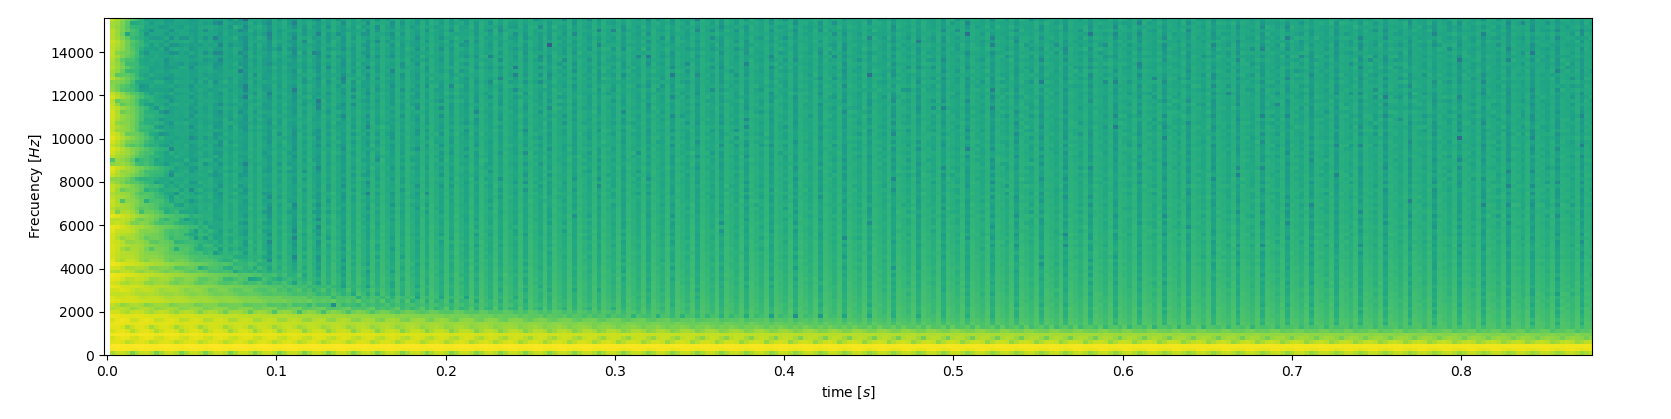
\includegraphics[width=1\textwidth]{ImagenesEjercicio4/espectroGuitar.PNG}
\caption{Espectrograma Guitarra.}
	\label{fig:especGuitar}
\end{figure}
\begin{figure}[H]
	\centering
	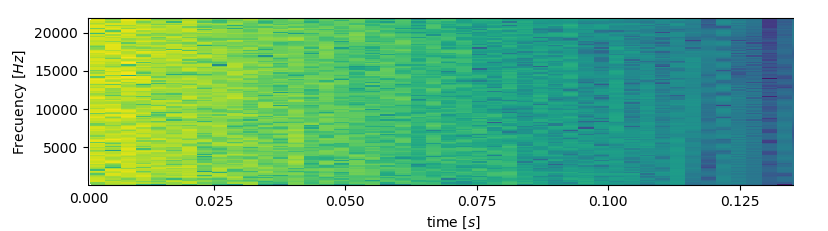
\includegraphics[width=1\textwidth]{ImagenesEjercicio4/espectroDrum.PNG}
\caption{Espectrograma Redoblante.}
	\label{fig:especdrum}
\end{figure}
Se puede diferenciar claramente que la guitarra cuenta con mayor densidad armonica de baja frecuencia al igual que se extiende considerablemente mas en el tiempo, mientra que el redoblante cuenta con mayor contenido de alta frecuencia y su duración es mucho menor.
\end{document}